\chapter{Introducción}

\label{introduccion}

\section{Ciencia  Ciudadana y Ciencia Abierta}

\begin{itemize}
   \item Ciencia Ciudadana
   \begin{itemize}
        \item Cómo participan los ciudadanos en la ciencia?        
        Esto de que hay que asignarles tareas acordes o darles una pequeña capacitación o ayuda en pantalla. Comunidades que hacen de soporte de voluntarios.
        \item De qué depende que un proyecto incluya ciencia ciudadana?
        Tipología de los proyectos de ciencia ciudadana, por ejemplo, que sea de educación, de investigación, que no cualquier proyecto puede tilizar ciencia ciudadana y no siempre se aplica en todo el proyecto. Muchas veces los ciudadanos colaboran con una parte.
   \end{itemize}   
   \item Ciencia Abierta   
   \begin{itemize}
        \item \item Por qué es importante la ciencia abierta? democracia y cuestiones políticas. Acceso público a la información de interés general. 
        \item Qué relación tiene con la ciencia ciudadana? Básicamente los participantes en proyectos de investigación de ciencia ciudadana lo hacen por interés en el tema de investigación. Es una buena práctica que una vez finalizada la investigación se haga una devolución de los resultados de la misma para que los ciudadanos participantes quienes estaban interesados en el tema de movida puedan ver los resultados de la investigación. Este tema está directamente relacionado con la ciencia abierta que básicamente es abrir los datos, resultados y procesos utilizados para conseguir resultados a el público general.
   \end{itemize}
\end{itemize}

\section{ Dispositivos Móviles y Android }
\begin{itemize}
	\item Distribución de dispositivos móviles entre la población
	cantidad de personas que tienen dispositivos móviles. Que porcentaje de la población representan. Zonas de concentración de dispositivos:cómo están distribuidos
	\item Características de los dispositivos móviles
	cámaras, micrófonos, conexiones a redes, posibilidad de transferencias de archivos, navegabilidad en la interfaz de aplicación. 
    \item Android 
    el sistema operativo. Licencia. Estructura. Versiones y lo que ello implica.
    \item Ejemplos de aplicaciones de ciencia ciudadana y dispositivos móviles 
    hablemos del ejemplo africano que no tenía palabras para que la población partipe sin necesidad de saber leer o escribir. AppEAR y Cazamosquitos. Ejemplo aplicado a salud Colombia
\end{itemize}

\section{ Frameworks }

\begin{itemize}
	\item Frameworks para construir aplicaciones
    \item Configuración de aplicaciones mediante archivos
\end{itemize}

\begin{figure}
\begin{center}
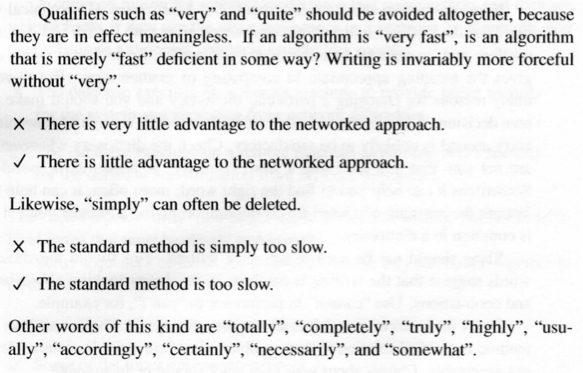
\includegraphics[width=0.8\textwidth]{00-introduccion/zobel-page-46}
\caption{Extracto del libro Writing for Computers Science de Justin Zobel}
\label{zobel-page-46}
\end{center}
\end{figure}

